\vspace{\baselineskip}
\hspace{0,5cm}La méthodologie mise en œuvre repose sur un ensemble d'étapes
soigneusement orchestrées : \\La collecte des données a été réalisée avec
rigueur et minutie. Une vaste compilation d'œuvres signées Molière ainsi que
celles d'autres auteurs contemporains a été rassemblée afin de constituer le
corpus de textes sur lequel s'appuie notre étude.  \\Le prétraitement des
données a été effectué avec une approche méthodologique précise. Des techniques
de prétraitement textuel sophistiquées ont été appliquées pour purifier les
données, éliminant ainsi les éléments superflus et les interférences
indésirables. Parmi ces techniques, on compte la suppression des stopwords, la
normalisation des mots et la lemmatisation.  \\L'analyse des caractéristiques
textuelles a été entreprise avec une attention particulière portée à chaque
auteur. Par le biais de techniques d'analyse textuelle avancées, notamment
l'analyse de fréquence des mots, l'exploration des n-grammes et l'évaluation de
la similarité, nous avons extrait et étudié en profondeur les traits
caractéristiques propres au style d'écriture de chacun.  \\La classification des
textes a constitué une étape cruciale de notre démarche.  Nous avons employé des
méthodes de classification établies, telles que les arbres de décision et les
algorithmes de classification bayésienne, pour attribuer à chaque segment de
texte son auteur d'origine, qu'il s'agisse de Molière ou d'un autre écrivain de
référence. 

\hspace{0,5cm}Notre expérience s'est divisée en deux axes. Le premier axe
consiste à déterminer comprendre et étudier le style d'écriture de Molière. Le
second axe consiste à déterminer les clusters de textes qui se ressemblent le
plus.

\hspace{0,5cm}Grâce à la bibliothèque \textbf{NLTK} et \textbf{WorldCloud}, nous
avons pu faire un nuage de mot pour le corpus de Molière. Un nuage de mots est
une manière de visualiser la fréquence des mots dans un corpus. Les mots
les plus fréquents sont présentés sous forme de nuage, où la taille du mot est
proportionnelle à sa fréquence. Cette représentation peut donner une vue
d'ensemble rapide des termes les plus courants dans le corpus de Molière. Pour
que l'analyse soit plus pertinente nous avons supprimé la prise en compte des
noms propres, qui sont uniques aux oeuvres.

\begin{figure}[htbp]
    \centering
    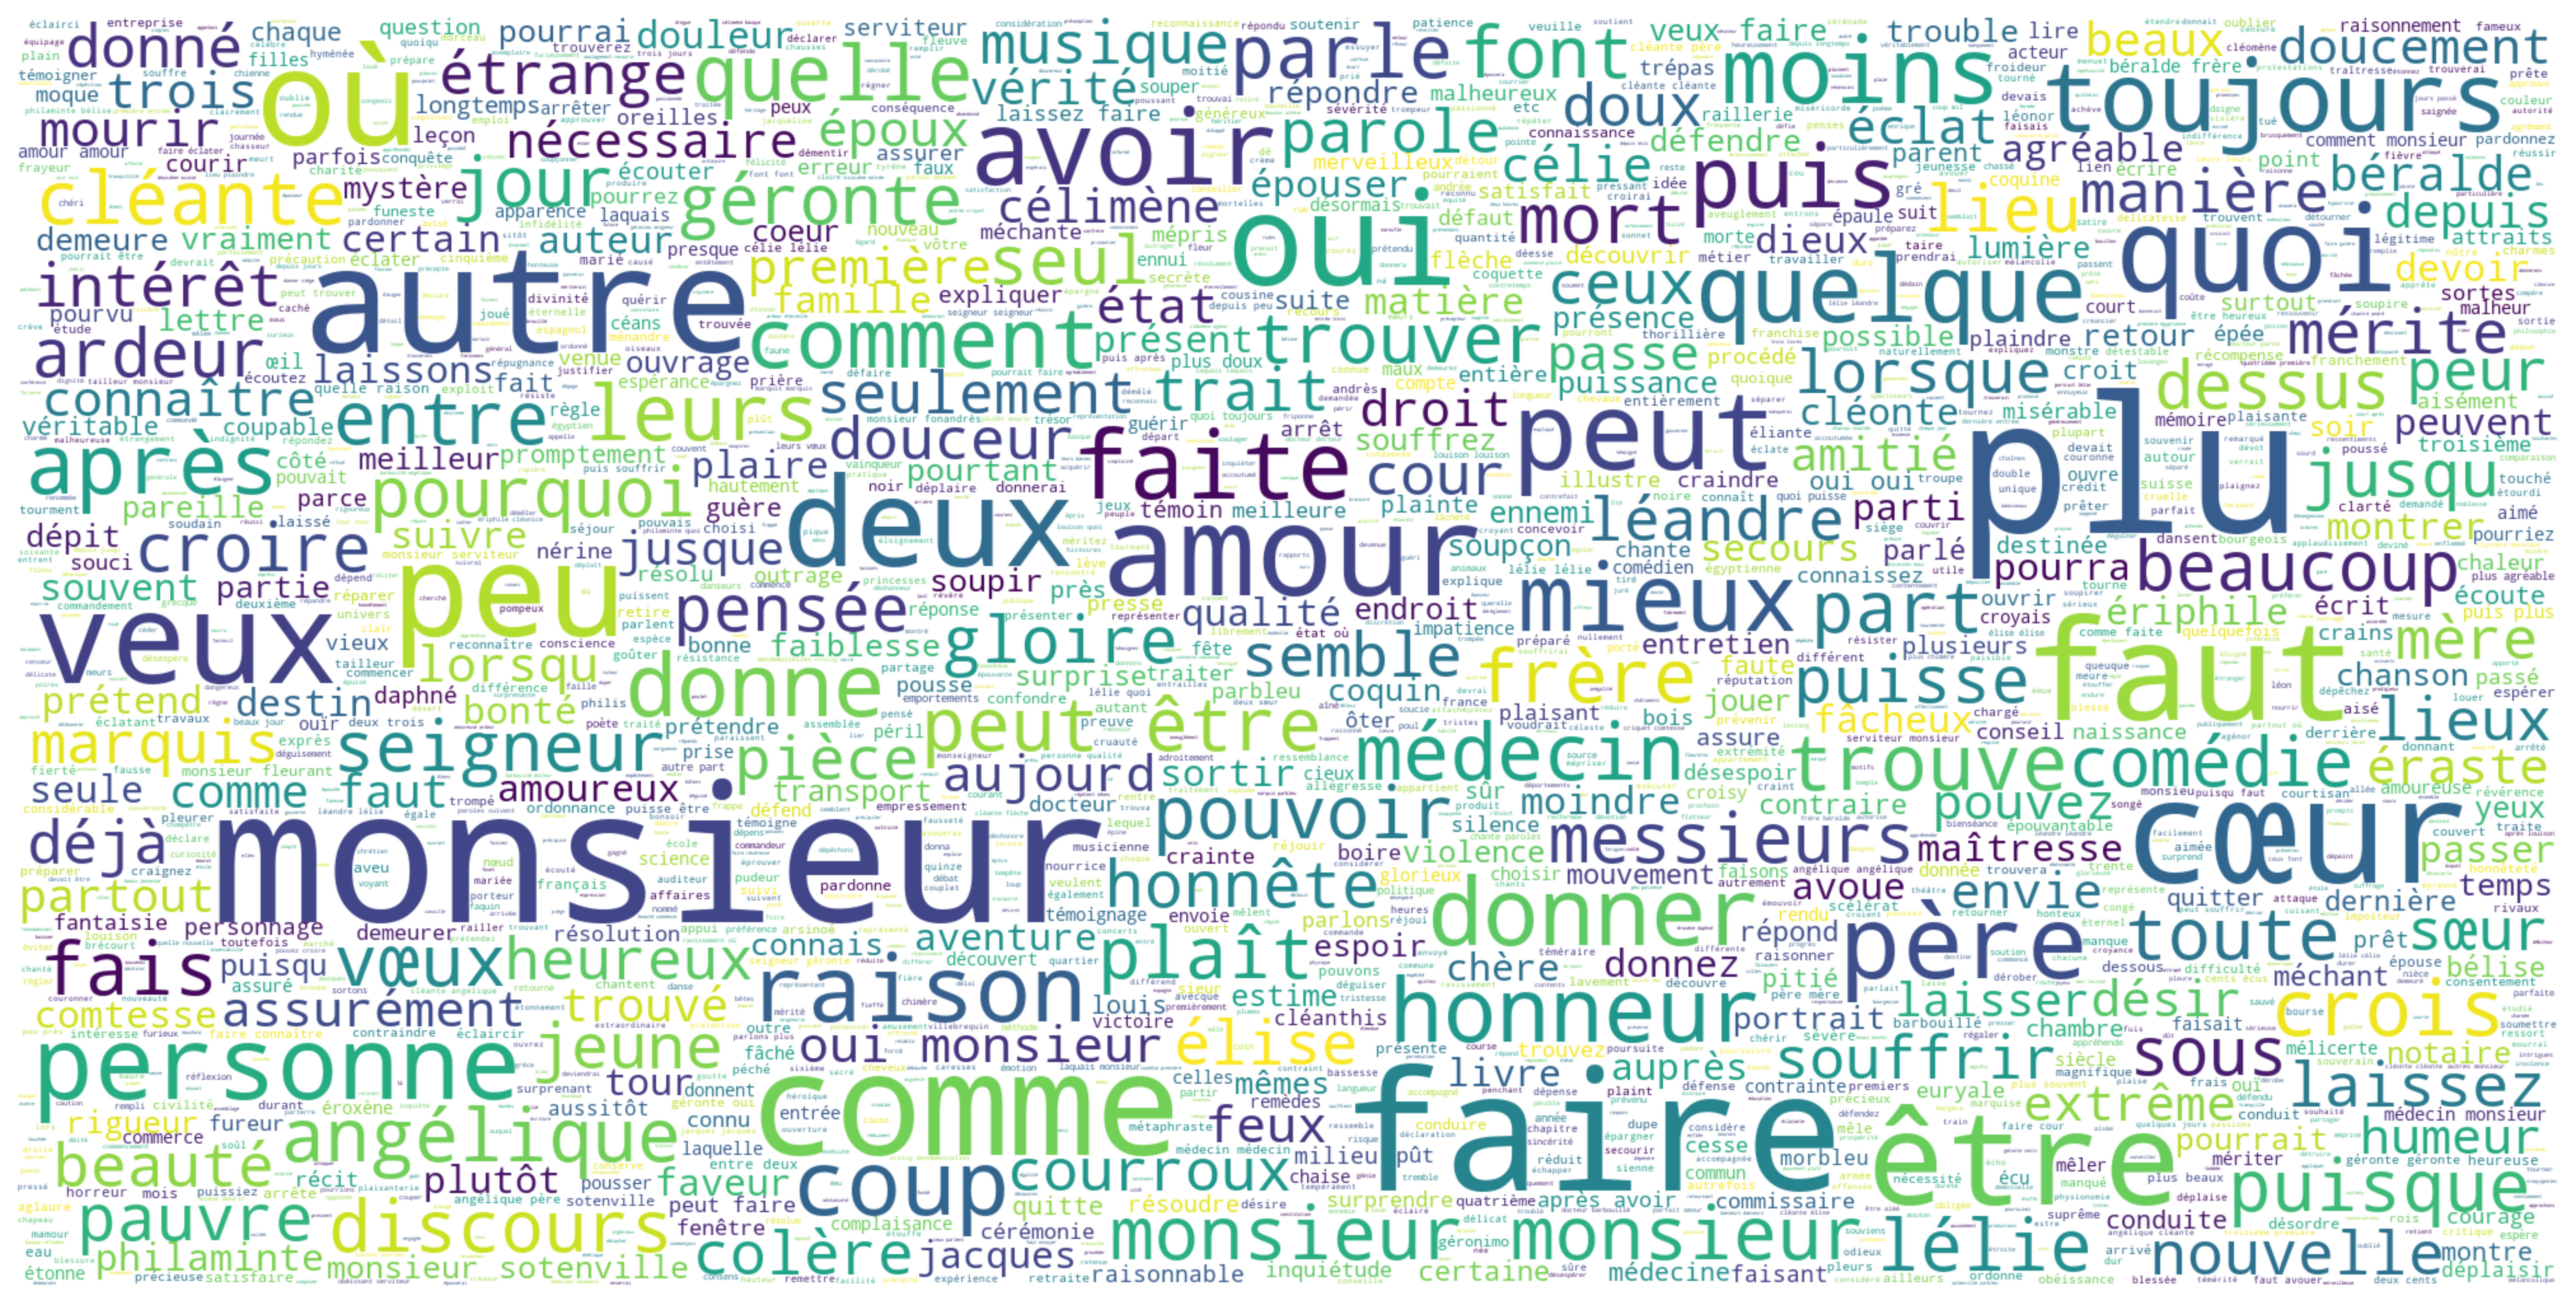
\includegraphics[width=15cm]{Ressources/nuage_sans_noms.png}
    \caption{Nuage de mots du corpus de Molière}
    \label{fig:images}
  \end{figure}

\vspace{\baselineskip}

\hspace{0,5cm}Grâce au nuage de mots, nous avions remarqué que le mot \textit{Monsieur}
revenait très souvent. Cette grande importance du mot \textit{Monsieur} dans le
nuage de mots révèle le vocabulaire et les règles d'écriture de l'époque.
\\Afin de mieux comprendre le style d'écriture de Molière, nous avons également
réaliser un histograme des mots les plus fréquents dans le corpus de Molière.
Pour rendre ce diagramme plus pertinent, nous avons décidé de ne pas prendre en
compte les noms de personnages mais également le mot \textit{Monsieur}.

\begin{figure}[htbp]
    \centering
    \includegraphics[width=13cm]{Ressources/diagr_sans_noms_mosn.png}
    \caption{Diagramme de mots du corpus de Molière sans le mot \textit{Monsieur}}
    \label{fig:images}
  \end{figure}

  \vspace{\baselineskip}

